%% 
%% Copyright 2007, 2008, 2009 Elsevier Ltd
%% 
%% This file is part of the 'Elsarticle Bundle'.
%% ---------------------------------------------
%% 
%% It may be distributed under the conditions of the LaTeX Project Public
%% License, either version 1.2 of this license or (at your option) any
%% later version.  The latest version of this license is in
%%    http://www.latex-project.org/lppl.txt
%% and version 1.2 or later is part of all distributions of LaTeX
%% version 1999/12/01 or later.
%% 
%% The list of all files belonging to the 'Elsarticle Bundle' is
%% given in the file `manifest.txt'.
%% 

%% Template article for Elsevier's document class `elsarticle'
%% with numbered style bibliographic references
%% SP 2008/03/01

%% Use the option review to obtain double line spacing
%% \documentclass[authoryear,preprint,review,12pt]{elsarticle}

%% Use the options 1p,twocolumn; 3p; 3p,twocolumn; 5p; or 5p,twocolumn
%% for a journal layout:
%% \documentclass[final,1p,times]{elsarticle}
%% \documentclass[final,1p,times,twocolumn]{elsarticle}
%% \documentclass[final,3p,times]{elsarticle}
%% \documentclass[final,3p,times,twocolumn]{elsarticle}
%% \documentclass[final,5p,times]{elsarticle}
%% \documentclass[final,5p,times,twocolumn]{elsarticle}

%% The amsthm package provides extended theorem environments
%% \usepackage{amsthm}

\newif\ifDRAFT
\DRAFTfalse
%\DRAFTtrue

\ifDRAFT
\documentclass[review,number,sort&compress,12pt]{elsarticle}
    %% The lineno packages adds line numbers. Start line numbering with
%% \begin{linenumbers}, end it with \end{linenumbers}. Or switch it on
%% for the whole article with \linenumbers.
%% \usepackage{lineno}
    \usepackage{lineno}
    \newcommand{\picwidth}{0.8\textwidth}
\else 
  \documentclass[final,5p,times]{elsarticle}
    \newcommand{\picwidth}{0.48\textwidth}
\fi

% packages
%\usepackage{fontspec}
%\setmainfont{Gulliver}

\usepackage{amsmath}
\usepackage{amssymb}
\usepackage{bm}
\usepackage{braket}
\usepackage{booktabs}
\usepackage{graphicx}
\usepackage{xcolor}
\usepackage{tikz}
\usetikzlibrary{patterns}
\usepackage{subcaption}
\usepackage{url}
\usepackage{setspace}
\usepackage{diagbox} % generate diagonal divided cell in table
\usepackage{float}
\usepackage{graphicx}
\usepackage{subcaption}
\floatplacement{figure}{H}

\usepackage[linesnumbered,ruled]{algorithm2e}
\usepackage{algpseudocode}
%\usepackage{mathalfa}
%\usepackage{mathrsfs}
\DeclareMathOperator*{\argmin}{argmin}
%\DeclareMathAlphabet{\mathcal}{OT1}{pzc}{m}{bf}
\usepackage[imagesright]{rotating}
%\usepackage{subfigure}
\captionsetup[subfigure]{labelformat=simple,labelsep=colon}
\renewcommand{\thesubfigure}{fig\arabic{subfigure}}



% new commands
\newcommand{\EQ}[1]{Eq.~(\ref{#1})}                
\newcommand{\EQUATION}[1]{Equation~(\ref{eq:#1})} 
\newcommand{\TWOEQS}[2]{Eqs.~(\ref{eq:#1})~and~(\ref{eq:#2})}  
\newcommand{\TWOEQUATIONS}[2]{Equations~(\ref{eq:#1})~and~(\ref{eq:#2})}  
\newcommand{\EQS}[1]{Eqs.~(\ref{#1})}             %-- Eqs. (refeqs)
\newcommand{\EQUATIONS}[1]{Equations~(\ref{#1})}  %-- Eqs. (refeqs)
\newcommand{\FIG}[1]{Fig.~\ref{#1}}               %-- Fig. refig
\newcommand{\FIGURE}[1]{Figure~\ref{#1}}          %-- Figure refig
\newcommand{\TAB}[1]{Table~\ref{#1}}              %-- Table tablref
\newcommand{\SEC}[1]{Section~\ref{#1}}               %-- Eq. (refeq)
\newcommand{\REF}[1]{Ref.~\citen{#1}}               %-- Eq. (refeq)
\newcommand{\BLUE}[1]{\textcolor{blue}{#1}}
\renewcommand{\vec}[1]{\boldsymbol{#1}} %vector is bold italic
\newcommand{\vd}{\bm{\cdot}} % slightly bold vector dot
\newcommand{\grad}{\vec{\nabla}} % gradient
\newcommand{\ud}{\mathop{}\!\mathrm{d}} % upright derivative symbol
\graphicspath{{../data/rendered/}}


\ifDRAFT
\doublespacing
\fi

\journal{STAT 713}
\usepackage{filecontents,catchfile}

\begin{document}
% \sloppy % prevent words spill into the margin
\begin{frontmatter}

\title{Dynamic Mode Decomposition as a Linear Model for Spatio-temporal Systems}

\author{Jeremy A. Roberts\corref{cor}}
\ead{jaroberts@k-state.edu}
\address{Department of Statistics, Kansas State University, Manhattan, KS 66506, USA}
\cortext[cor]{Corresponding author}

% 100–300 word summary of your report
\begin{abstract}
Dynamic Mode Decomposition (DMD) is a method for decoupling the spatio-temporal dynamics of an observed system.
Here, DMD was used to produce spatio-temporal basis functions for the analysis of spatially-discrete but temporally
continuous processes (measured at discrete time intervals).
The basis use of DMD for producing basis vectors is prescribed, and a key features of the method are highlighted.
The method is used to form basis vectors for a standard, linear model of temperature measurements distributed across the United States.
The model is compared to a polynomial method, and the results indicate the DMD basis vectors capture spatio-temporal variation more efficiently.
Though preliminary, the work suggests that DMD may find use in spatio-temporal, statistical modeling.
\end{abstract}

\begin{keyword}
 spatio-temporal basis functions \sep rank reduction \sep dynamic mode decomposition.
\end{keyword}
\end{frontmatter}

\ifDRAFT
\linenumbers
\fi

%%%%%%%%%%%%%%%%%%%%%%%%%%%%%%%%%%%%%%%%%%%%%%%%%%%%%%%%%%%%%%%%%%%%%%%%%%%%%%%%
\section{Introduction}
\label{sec:introduction}
% 500--1000 words

Many of the largest data sets in this era of ``big data'' are generated from measurements of processes that evolve in space and time.
These measurements may be physical or simulated, but the often inseparable dependence of the latent process (i.e., the ``true'' but unknown process) on space and time makes the development of satisfactory statistical models for the data a challenging task.
A rich literature exists on spatio-temporal, statistical models (see, e.g., Refs. \cite{cressie2011sst} and \cite{wikle2019sts}).
Such models can be categorized as descriptive or dynamic.  
Descriptive models define a mean and covariance, often via kriging, and are consistent with the spirit of general linear models.  
Dynamic models assume that evolution in space and time follow some explicity defined, usually Markovian, process and, hence, appear to live somewhat outside the domain of general linear models (though the processes assumed can be and often are linear).

For both descriptive and dynamic models, the construction of suitable basis vectors in space, time, or both is often important for reducing the dimension of the problem.
With descriptive models, use of a low-rank basis, as in fixed-rank kriging, leads to smaller, more practical covariance matrices.
For dynamic models, the governing process can be projected onto a low-rank basis that captures the dominant characteristics of the system.
Common basis functions including linear, wavelet, Gaussian, and sinusoidal shapes in both space and time, and these can be combined via Kronecker products to produce a spatio-temporal basis.
Alternative basis vectors known as empirical orthogonal functions (EOFs) can be derived directly from the spatio-temporal observations through use of the singular-value decomposition of the space-averaged or time-averaged observations.
Such inherently discrete vectors can be used as continuous functions with appropriate interpolation.

The effort described here explored the use of dynamic-mode decomposition (DMD) \cite{schmid:hal-01053394} to produce spatially-discrete, temporally continuous basis functions for use in spatio-temporal, statistical models.
The DMD algorithm was first reported as a technique by which to analyze spatio-temporal structures in complex fluid flows \cite{schmid:hal-01053394, schmid2010dynamic}.
Several extensions to DMD and its connection to the much older Koopman operator theory have been well described in a recent monograph \cite{kutzbook}.  
Basically, given a nonlinear, dynamical system
\begin{equation}
  \frac{d\mathbf{z}}{dt} = \mathbf{f}(\mathbf{z}) \, ,
  \label{eq:dynamicalsystem}
\end{equation}
the infinite dimensional but linear Koopman operator $\mathcal{K}$ satisfies the relationship $\mathcal{K}\mathbf{g}(\mathbf{z}) = \mathbf{g}(\mathbf{f}(\mathbf{z}))$ for some measurement function $\mathbf{g}$.
If the eigenfunctions of $\mathcal{K}$ are known, then measurements $\mathbf{g}(\mathbf{z})$ made from the original, nonlinear system can instead be defined directly using an eigenfunction expansion and known initial conditions.
In practice, neither $\mathcal{K}$ nor its eigenfunctions are generally accessible, and finite-dimensional approximations are sought; the DMD algorithm provides this approximation, and the resulting eigenmodes it produces form the basis vectors used in the present work.

To limit the scope of the study, the generated basis vectors were applied only within a standard, linear model (i.e., fixed effects with uncorrelated, normally-distributed errors). Moreover, the development is limited to those problems in which measurements $z_{ij}$ are made on a fixed, regular, spatio-temporal grid, i.e., for spatial points $\mathbf{r}_i, i = 1, 2, \ldots m$ and times $t_j, j = 1, 2, \ldots n$. 
Here, each spatial coordinate $\mathbf{r}_i$ is treated as a vector to account for more than one dimension, e.g., $\mathbf{r}_i = [x_i, y_i]$ in two-dimensional, Cartesian coordinates.
In other words, the entire set of measurements can be viewed as a matrix $\mathbf{Z} \in \mathbb{R}^{m\times n}$ with elements $z_{ij}$. 
An alternative representation is the reshaped, $mn \times 1$ vector $\boldsymbol{\zeta} = [z_{11}, z_{21}, \ldots z_{m1}, z_{12}, \ldots, z_{mn}]$.
With this representation, let
\begin{equation}
 \boldsymbol{\zeta} = \boldsymbol{\Psi}\boldsymbol{\beta} + \boldsymbol{\varepsilon} \, ,
 \label{eq:linmodel}
\end{equation}
where $\boldsymbol{\varepsilon} \sim N(0, \mathbf{I}\sigma^2_{\varepsilon})$ and the columns $\boldsymbol{\psi}_k$ of the design matrix $\boldsymbol{\Psi}$ are basis vectors.

Although the DMD algorithm provides a deterministic way by which to define $\mathbf{\psi}$, there are many ways to choose how many modes to use, which modes to use, and how to combine the selected modes.
A key issue addressed in the study is to explore statistical metrics for choosing the number of basis functions to use and how to combine them in an optimal way.
To aid in this exploration, sea-surface temperature (SST) anomaly data as provided by Ref.~\cite{wikle2019sts} were adopted for all analyses.
Because only one set of data was explored, this study is naturally preliminary in nature, but the results suggest that DMD may be a very powerful way to incorporate the leading dynamics of a system into a basis used for fixed effects (as studied here) and, possibly, random effects in general linear models.


%%%%%%%%%%%%%%%%%%%%%%%%%%%%%%%%%%%%%%%%%%%%%%%%%%%%%%%%%%%%%%%%%%%%%%%%%%%%%%%%
\section{Methods}
\label{sec:methods}
% 500--1000 words

\subsection{Dynamic Mode Decomposition} 

Central to the analysis presented here is the DMD algorithm.
Despite its connections to the more general Koopman theory, DMD can be motivated in somewhat simpler (albeit, heuristic) terms by adapting the presentation of Ref.~\cite{kutzbook}.
Consider again a dynamical system described by Eq.~(\ref{eq:dynamicalsystem}), where $\mathbf{z} \in \mathbb{R}^n$ is the $n$-dimensional state vector at time $t$.
Suppose there exists some linear operator $\mathcal{A}$ such that
\begin{equation}
 \frac{d \mathbf{z}}{dt} = \mathcal{A} \mathbf{z} \, .
 \label{eq:approxdynamicalsystem}
\end{equation}
One might note that this $\mathcal{A}$ represents the Koopman operator for the measurement function $\mathbf{g}(\mathbf{z}) = \mathbf{z}$ and is likely not known explicitly.
However, let the system be observed, leading to a sequence of observations of the state vector in time, i.e., $\mathbf{Z} = [\mathbf{z}_{1}, \mathbf{z}_{2}, \ldots \mathbf{z}_{n}$], where the $m$-vector $\mathbf{z}_{j}$ is the $j$th column of $\mathbf{Z}$. 
For simplicity, assume these observations are taken at equally-spaced times $t_0, t_1, \ldots t_n$ with $t_{i+1} = t_i + \Delta t$.  
Now, let there be some, possibly approximate, linear mapping $\mathbf{z}_{j+1} \approx \mathbf{A}\mathbf{z}_{j}$, or \begin{equation}
   \mathbf{Z}_+ \approx \mathbf{A}\mathbf{Z}_- \, ,
   \label{eq:linearmapping}
\end{equation}
where
\begin{equation}
  \mathbf{Z}_+ =  [\mathbf{z}_{2},\mathbf{z}_{3}, \ldots,\mathbf{z}_{n}] \, ,
\end{equation}
and
\begin{equation}
 \mathbf{Z}_- =  [ \mathbf{z}_{1},\mathbf{z}_{2},\ldots, \mathbf{z}_{n-1}] \,  .                                                                                                           
\end{equation}
Since the solution to Eq.~(\ref{eq:approxdynamicalsystem}) is $\mathbf{z}(t) = e^{\mathcal{A}t}\mathbf{z}(0)$, $\mathbf{A}$ is the discrete-time approximation to $e^{\mathcal{A}\Delta}$.
In addition, the  eigenvalues of $\mathbf{A}$ are related to the continuous-time eigenvalues $\omega_i$ of $\mathcal{A}$ by 
\begin{equation}
 \omega_i = \frac{\ln{(\lambda_i)}}{\Delta} \, .
\end{equation}
Corresponding to $\lambda_i$ is the eigenvector $\boldsymbol{\varphi}_i$ of $\mathbf{A}$, and, hence,
\begin{equation}
 \mathbf{z}(t) \approx \sum^{n-1}_{i=1} \boldsymbol{\varphi}_i e^{\omega_i t} b_i = \boldsymbol{\Phi}e^{\boldsymbol{\Omega}t}\mathbf{b} \, . 
 \label{eq:dmdreconstruction}
\end{equation}
Although there is no unique way to define the weights $\mathbf{b}$, one can satisfy $\mathbf{z}_1 = \boldsymbol{\Phi}\mathbf{b}$  in a least-squares sense by defining
\begin{equation}
 \mathbf{b} = \boldsymbol{\Phi}^{\dagger} \mathbf{z}_1 \, ,
 \label{eq:amplitudes}
\end{equation}
where $\dagger$ indicates the pseudoinverse. 

In general, there is no $\mathbf{A}$ that satisfies Eq.~(\ref{eq:linearmapping}) exactly.
However, the best-fit operator (in the Frobenius-norm sense) is $\mathbf{A} = \mathbf{Z}_+ \mathbf{Z}^{\dagger}_-$.
In practice, the (thin) singular value decomposition
\begin{equation}
 \mathbf{Z}_-=\mathbf{U\Sigma V}^*  \, ,
\end{equation}
is used to define 
\begin{equation}
 \mathbf{Z}^{\dagger}_- = \mathbf{V}\boldsymbol{\Sigma}^{-1}\mathbf{U}^* \, ,
\end{equation}
where $\mathbf{U} \in \mathbb{C}^{m\times n}$, $\mathbf{V} \in \mathbb{C}^{n\times n}$, and $\boldsymbol{\Sigma} \in \mathbb{C}^{n\times n}$.  
Then the best-fit operator is
\begin{equation}
 \mathbf{A} = \mathbf{Z}_+ \mathbf{V} \boldsymbol{\Sigma}^{-1}\mathbf{U}^* \, .
\end{equation}
The columns of $\mathbf{U}$ are readily interpreted as the eigenvectors of the matrix $\mathbf{Z}_{-} \mathbf{Z}_{-}^* \in \mathbb{R}^{m\times m}$, which is strongly related to the spatial covariance matrix corresponding to the first $n-1$ measurements.
Consequently, the columns of  $\mathbf{U}$ represent the principal directions that account for time-averaged, spatial variation (without detrending and scaling) and, hence, are strongly related to EOFs \cite{wikle2019sts}.


Because $\mathbf{A}$ can be intractably large, the low-rank approximation
\begin{equation}
 \tilde{\mathbf{A}} = \mathbf{U}^*_r \mathbf{A} \mathbf{U}_r = \mathbf{U}^*_r \mathbf{Z}_+ \mathbf{V}_r\boldsymbol{\Sigma}_r^{-1} \, ,
 \label{eq:lowrank}
\end{equation}
is formed, where $\boldsymbol{\Sigma}_r \in \mathbb{C}^{r\times r}$ is a diagonal matrix containing the largest $r < n$ singular values, and  $\mathbf{U}_r, \mathbf{V}_r \in \mathbb{C}^{n\times r} $ contain the corresponding columns of $\mathbf{U}$ and $\mathbf{V}$.  
Finally, with the eigendecomposition $\tilde{\mathbf{A}}\mathbf{W} = \mathbf{W}\boldsymbol{\Lambda}$, the diagonal elements $\lambda_i$ of $\boldsymbol{\Lambda}$ are the leading $r$ eigenvalues of $\mathbf{A}$ with the corresponding eigenvectors (often called DMD modes)
\begin{equation}
 \boldsymbol{\Phi} = \mathbf{Z}_+ \mathbf{V}_r\boldsymbol{\Sigma}_r^{-1}\mathbf{W} \, .
\end{equation}
The reduced rank $r$ selected impacts the overall accuracy of the DMD reconstruction defined by Eq.~(\ref{eq:dmdreconstruction}). 
One way to select $r$ is to use the optimal hard threshold for singular values \cite{gavish2014optimal}, which provides the best denoising of a set of measurements subject to known, independently- and normally-distributed noise---precisely as assumed in Eq.~(\ref{eq:linmodel}).  

With each eigenvector $\boldsymbol{\phi}_k$ and eigenvalue $\lambda_k$ of $\mathbf{A}$, one can construct the spatio-temporal basis vector
\begin{equation}
  \boldsymbol{\psi}_k = 
    [\varphi_{ki} e^{\omega_k t_j} \, \text{for} \, i =1\ldots n \, \text{for} \, j = 1\ldots m]' \, ,
\end{equation}
which are the columns of $\boldsymbol{\Psi}$ as used in the linear model defined by Eq.~(\ref{eq:linmodel}).
In general, the columns of $\boldsymbol{\Psi}$ are not orthogonal, which leads to collinearity and, possibly, lower predictive accuracy with increased rank.  
Moreover, the basis vectors can be complex valued, which indicates oscillatory dynamics in the system and, in principle, may lead to  numerical challenges if the observable state is a physical (i.e., real-valued) quantity.
However, complex modes always appear in conjugate pairs. 
Hence, if both modes are included in the basis, the opposing, imaginary components will cancel upon projection of a real-valued quantity onto the basis in the absence of roundoff errors.
In other words, the real part of the conjugate pair may be kept as one basis vector, and complex values can be eliminated altogether from the final, linear model\footnote{In practice, 128-bit, complex arithmetic with the additional degrees of freedom offered by the conjugate modes may actually improve accuracy a bit.}.

Given the basis $\boldsymbol{\Psi}$, the maximum-likelihood estimates of the parameters $\boldsymbol{\beta}$ and $\sigma^2_{\varepsilon}$ of Eq.~(\ref{eq:linmodel}) can be made.
These estimates provide a more rigorous alternative to the coefficient values implied by Eq.~(\ref{eq:amplitudes}).  
A separate issue is decide which columns of the basis $\boldsymbol{\Psi}$ to use in the regression analysis.
Because these columns are not orthogonal (i.e., they are collinear), inclusion of one additional basis vector generally changes the impact of each other basis vector.
Past work applied an approximate, sparsity-promoting technique equivalent to lasso-regression for selecting a subset of modes to include followed by a standard, least-squares fit of the data to those modes \cite{jovanovic}.
For the present work, the number of modes computed (i.e., the rank $r$ in Eq.~\ref{eq:lowrank}) was fixed, and all modes computed were included in the basis.


%%%%%%%%%%%%%%%%%%%%%%%%%%%%%%%%%%%%%%%%%%%%%%%%%%%%%%%%%%%%%%%%%%%%%%%%%%%%%%%%
\section{Results}
\label{sec:results}
% 500--1000 words

To illustrate the use of DMD for constructing basis functions, a statistical model was constructed for the maximum temperature recorded at each of over 100 weather stations located in the midwestern and southeastern United Stated. 
The data used is distributed with the software developed in support of Ref.~\cite{wikle2019sts} but was originally extracted from the National Oceanic Atmospheric Administration (NOAA) IRI/LDEO Climate Data Library.
The specific case studied is an adaptation of an exercise presented in Ref.~\cite{wikle2019sts} in which spatial, temporal, and spatio-temporal basis functions are explored for predicting the maximum temperature at arbitrary points in space and time.
However, because DMD produces spatially-discrete basis vectors, the exercise was modified to produce spatially-discrete models.

Specifically, models were developed for the maximum temperature at each station during July of 1993.
To simplify the application of DMD, data was included only from the 132 stations for which measurements were made on each of the 31 days.
Two DMD-based models were constructed, each using three spatio-temporal basis functions; in all cases, the SVD rank $r$ was set to 5, but elimination of complex conjugate pairs resulted in just three vectors.
In other words, each model had the form
\begin{equation}
 \boldsymbol{\zeta} \sim \mathcal{N}(\boldsymbol{\Psi}\boldsymbol{\beta}, \sigma^2 \mathbf{I}) \, ,
\end{equation}
where, of note, $\beta_0$ does {\it not} correspond to an intercept.
The first DMD model, referred to as {\tt dmd-full}, was constructed using all 31 days of measurements, both for the basis definition and the regression (using {\tt lm}).  
The second DMD model, referred to as {\tt dmd-partial}, was constructed using the first 28 days of measurements, again for the basis and regression.
For comparison (albeit, an uninspiring one), a polynomial model was used of the form
\begin{equation}
\begin{split}
 \zeta_k = \beta_0 &+ \beta_1 t_k + \beta_2 a_k + \beta_2 o_k + \beta_3 t_k a_k \\
                   &+ \beta_4 t_k o_k + \beta_5 a_k o_k  + \varepsilon \, ,
\end{split}
\end{equation}
where $t_k$, $a_k$, and $o_k$ represent time, latitude, and longitude of the $k$th measurement, and $\varepsilon \sim N(0, \sigma^2)$.
This model was fitted using the same partial or full set of data ({\tt poly-partial} and {\tt poly-full}).

Shown in Figs.~\ref{fig:dmd_full}--\ref{fig:poly_part} are the predicted, maximum temperatures at station 14943.
Additionally, the 95\% prediction intervals are shown.


\begin{figure}[h]
 \centering
 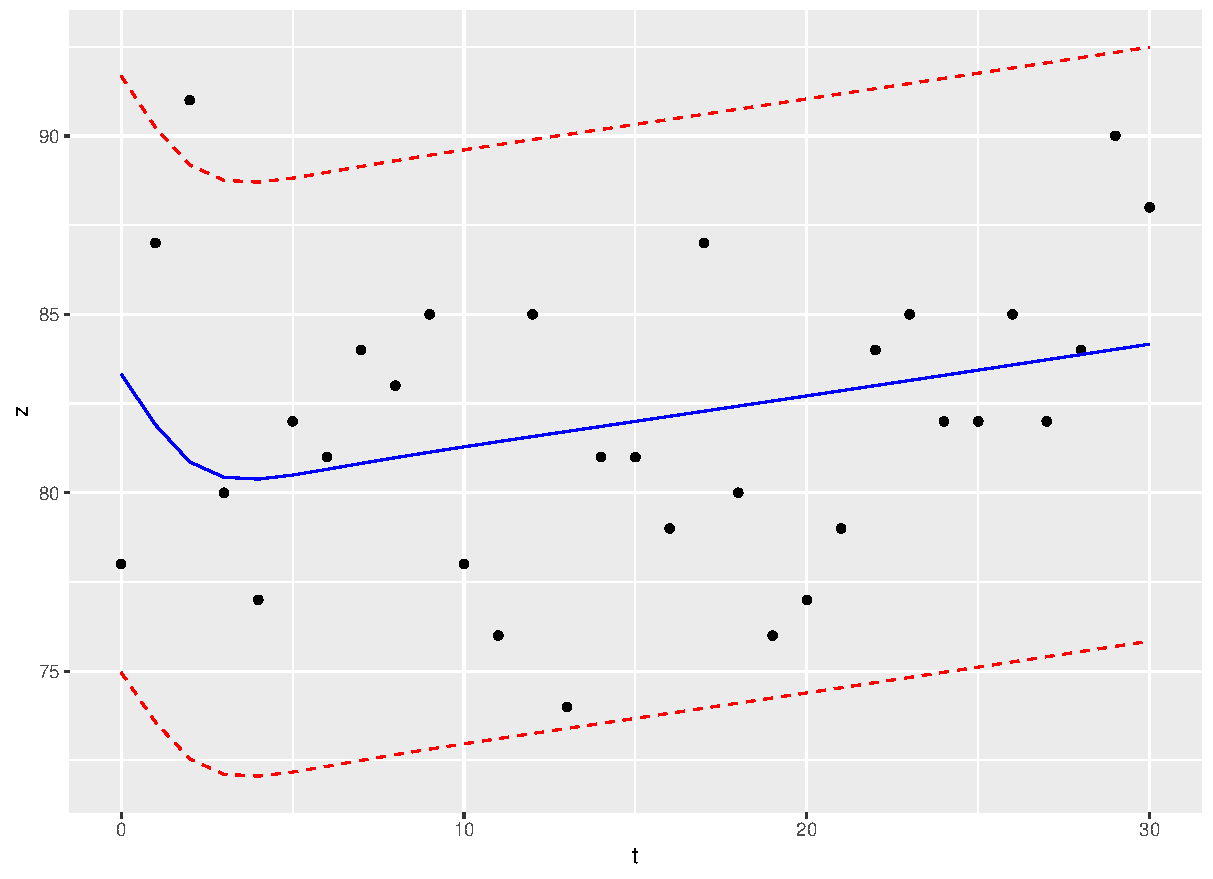
\includegraphics[width=0.5\textwidth]{../code/plot_dmd_full.pdf}\\
   \caption{Prediction and prediction intervals for {\tt dmd-full}.}
  \label{fig:dmd_full}
\end{figure}
\begin{figure}[h]
 \centering
 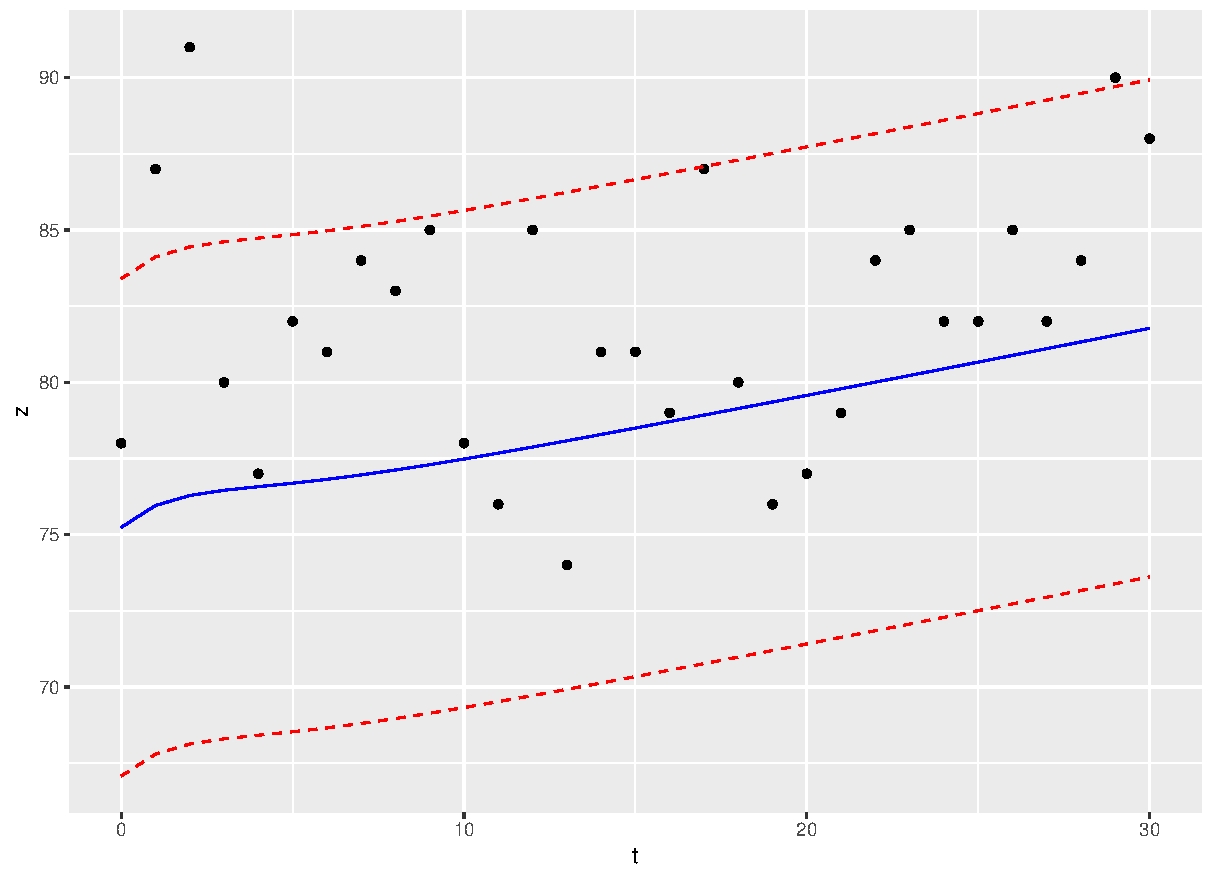
\includegraphics[width=0.5\textwidth]{../code/plot_dmd_part.pdf}\\
   \caption{Prediction and prediction intervals for {\tt dmd-part}.}
  \label{fig:dmd_part}
\end{figure}
\begin{figure}[h]
 \centering
 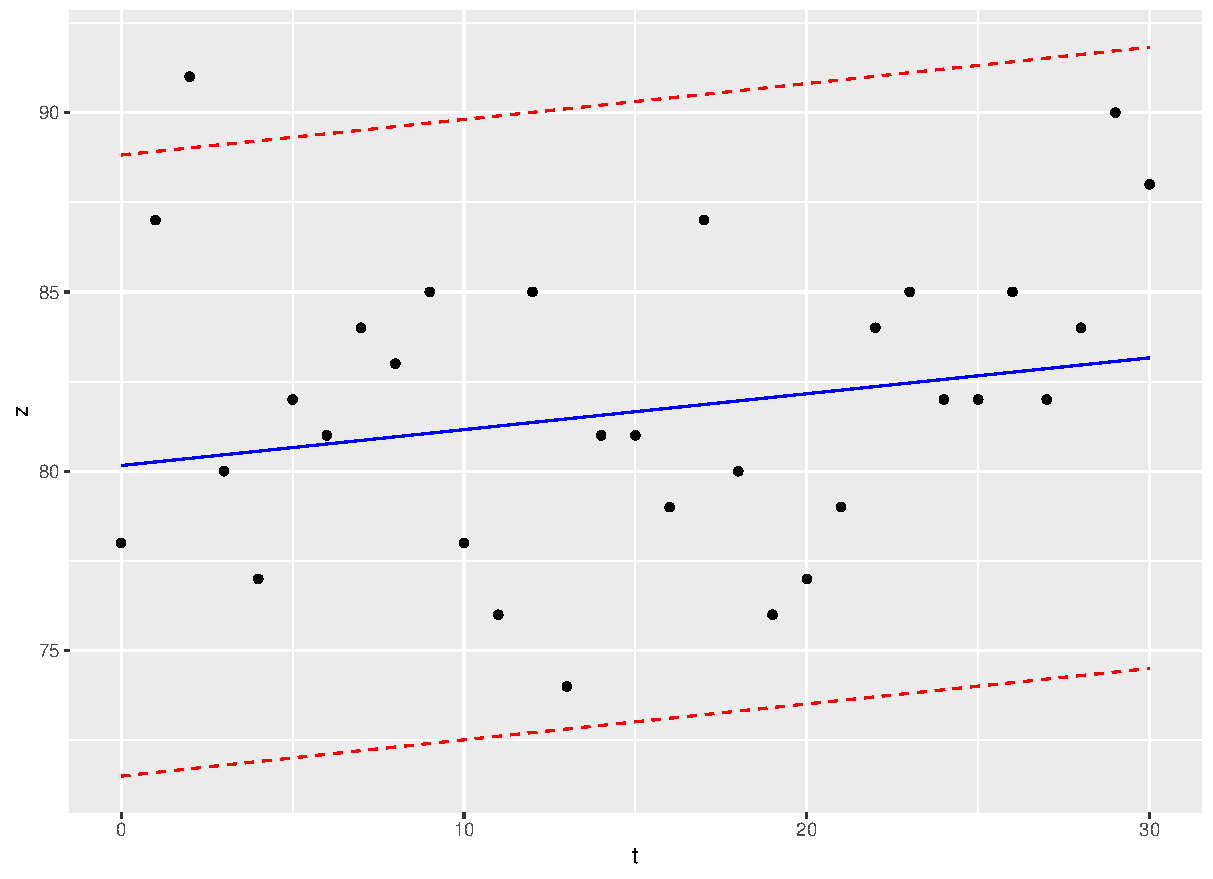
\includegraphics[width=0.5\textwidth]{../code/plot_poly_full.pdf}\\
   \caption{Prediction and prediction intervals for {\tt poly-part}.}
  \label{fig:poly_full}
\end{figure}
\begin{figure}[h]
 \centering
 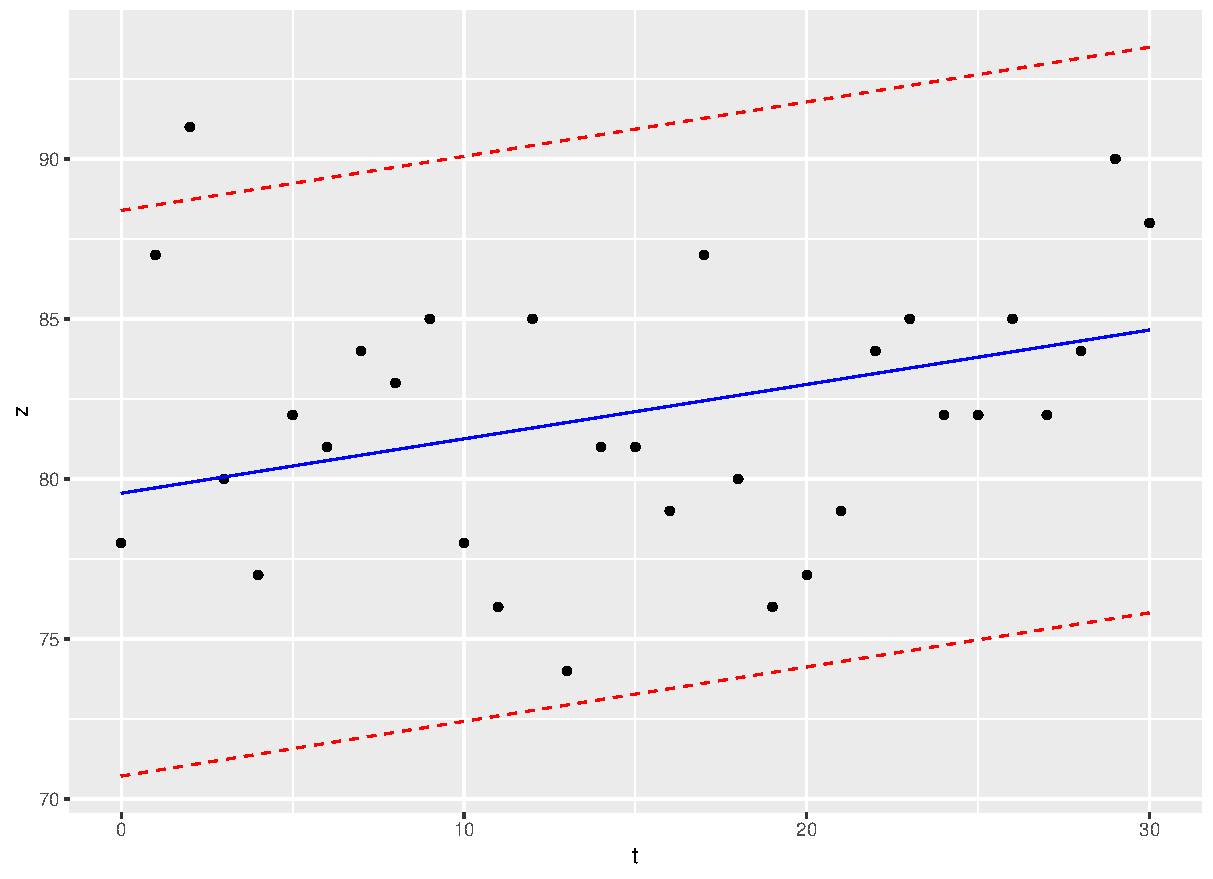
\includegraphics[width=0.5\textwidth]{../code/plot_poly_part.pdf}\\
   \caption{Prediction and prediction intervals for {\tt poly-part}.}
  \label{fig:poly_part}
\end{figure}

All four models appear to capture the observations reasonably well.
Of some interest is that each of the DMD covariates (the basis vectors) had corresponding $p$ values below $10^{-5}$, indicates their apparent importance.



%%%%%%%%%%%%%%%%%%%%%%%%%%%%%%%%%%%%%%%%%%%%%%%%%%%%%%%%%%%%%%%%%%%%%%%%%%%%%%%%
\section{Discussion}
\label{sec:discusion}
% 500--1000 words

Dynamic mode decomposition was shown to generate spatio-temporal basis functions for discrete-space, continuous-time modeling.
The analysis described is very preliminary, but the results demonstrate that the basis functions produced lead to functioning models.
The mechanics of the process (evaluation of the vectors for different times, etc.) requires further development to facilitate continued study.
However, the process has been implemented entirely in R, and so continued work should be reasonably straightforward.

Further work should pursue the use of the DMD basis in conjunction with continuous treatments of space. 
In particular, it seems plausible the DMD modes could be used directly to inform spatio-temporal correlation functions for Gaussian-process models.
Finally, based on the literature surveyed so far, it does not seem DMD has been applied {\it by name} in the statistics community, but the similarity between it and more advanced spatio-temporal models suggests that there may be significant overlap between DMD and other methods (but this has not yet been identified).

\section*{References}
\bibliographystyle{elsarticle-num} 
\bibliography{references}

\end{document}
